\begin{frame}[fragile]{Lecture et écriture de fichier (\texttt{cat})}
    \texttt{cat f1 f2 f3}~... : concatène le contenu des fichiers en entrée et les écrit dans la sortie standard.
    
    \subtt{Exemple}
    
    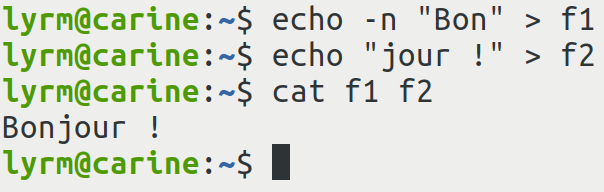
\includegraphics[width=0.5\textwidth]{slides/images/shell_cat.png}
    
    \pause\subtt{Pseudo-code}

    Pour chaque fichier en entrée : 
    \begin{itemize}[label=\small\ding{114}]
        \item ouvrir le fichier
        \item le lire et l'écrire sur la sortie standard
        \item fermer le fichier
    \end{itemize}
\end{frame}

\begin{frame}[fragile]{Lecture et écriture de fichier (\texttt{cat})}
    \begin{lstlisting}
        type file_descr         (* descripteurs de fichiers *)
        val stdin : file_descr  (* entree standard *)
        val stdout : file_descr (* sortie standard *)
        val stderr : file_descr (* sortie d'erreur standard *)
        
        type open_flag = (* modes d'ouverture *)
            | O_RDONLY  | O_WRONLY | O_RDWR
            | O_CREAT   | O_TRUNC 
         (* |.. et tous les autres  *)
        type file_perm = int (* droits (Ex : 0o777) *)
        
        val openfile : 
            string -> open_flag list -> file_perm -> file_descr
        val close : file_descr -> unit
        val read : file_descr -> bytes -> int -> int -> int
        val single_write : file_descr -> bytes -> int -> int -> int
    \end{lstlisting}
\end{frame}

\begin{frame}[fragile]{OCaml vs C : \texttt{write}}
    \begin{lstlisting}
        val single_write : file_descr -> bytes -> int -> int -> int    
    \end{lstlisting}
    
    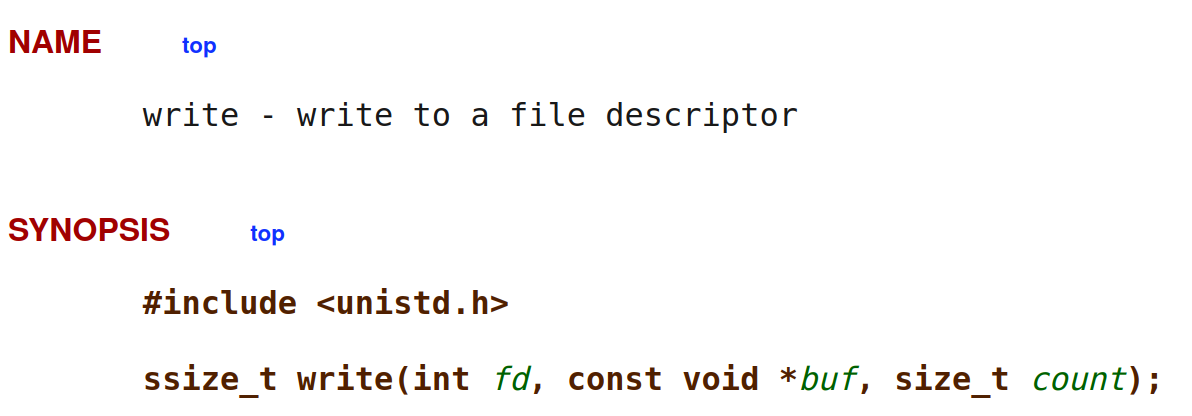
\includegraphics[width=0.8\textwidth]{slides/images/c_api_write.png}
\end{frame}

\begin{frame}[fragile]{OCaml vs C : \texttt{openfile}}
    \begin{lstlisting}
       val openfile : 
            string -> open_flag list -> file_perm -> file_descr
     \end{lstlisting}
    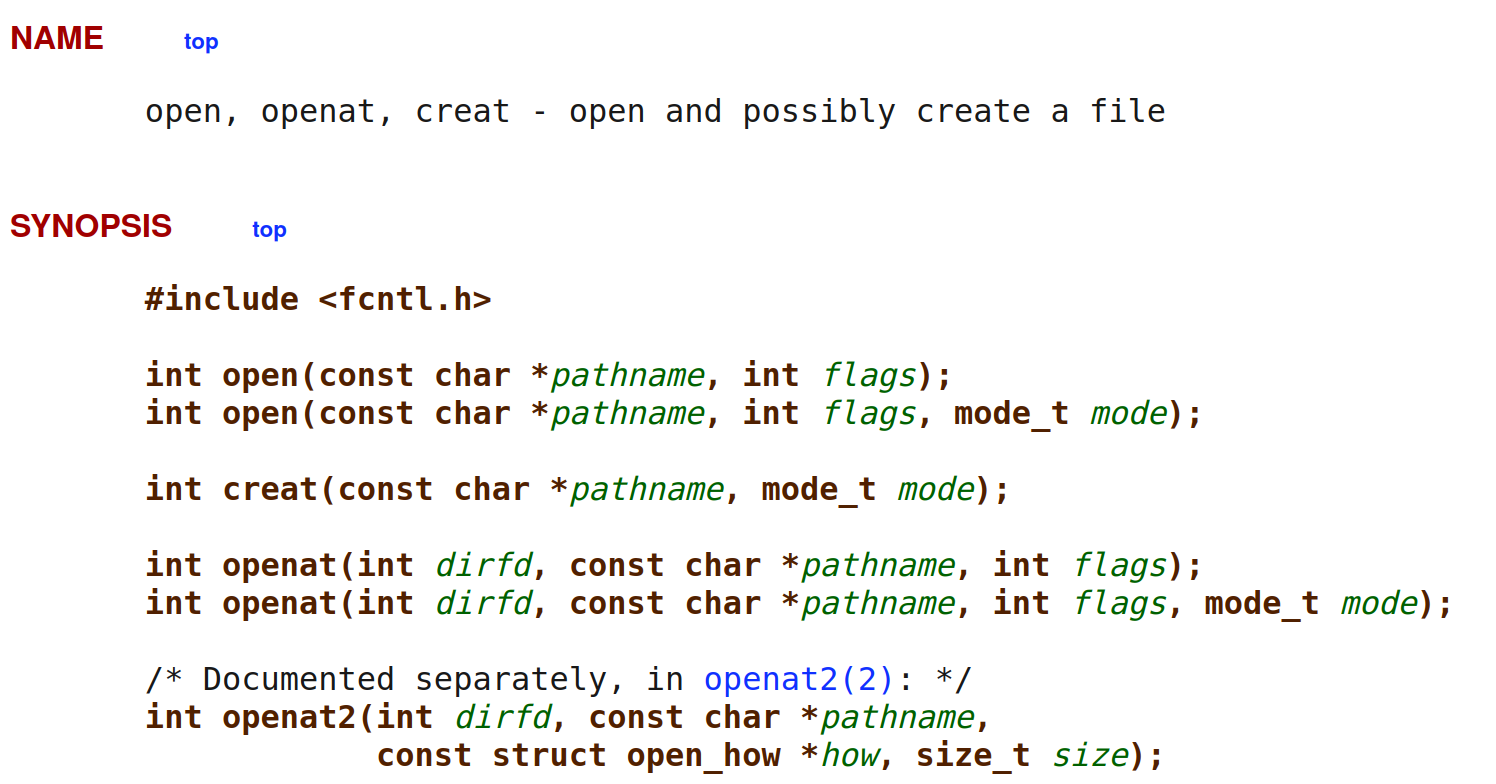
\includegraphics[width=\textwidth]{slides/images/c_api_open.png}
\end{frame}

\begin{frame}[fragile]{Lecture et écriture de fichier (\texttt{cat})}
     \begin{itemize}[label=\small\ding{114}]
         \item pour lire un fichier
             \begin{lstlisting}
                    Unix.openfile filename [O_RDONLY] 0
             \end{lstlisting}
         \item écrire en créant ou en effaçant un fichier existant
             \begin{lstlisting}
                Unix.openfile filename 
                    [O_WRONLY; O_TRUNC; O_CREAT] 0o666
            \end{lstlisting}
        \item écrire du code exécutable
             \begin{lstlisting}
                Unix.openfile filename 
                    [O_WRONLY; O_TRUNC; O_CREAT] 0o777
            \end{lstlisting}
        \item ajouter des données à la fin d'un fichier existant ou le créer vide sinon
             \begin{lstlisting}
                Unix.openfile filename 
                    [O_WRONLY; O_APPEND; O_CREAT] 0o666
            \end{lstlisting}
     \end{itemize} 
\end{frame}

\begin{frame}[fragile]{Lecture et écriture de fichier (\texttt{cat})}
    \begin{itemize}[leftmargin=-10pt]
        \item<2->
            \begin{lstlisting}[basicstyle=\footnotesize\ttfamily]
                let exec_cmd cmd = match cmd with 
                  | Cat files -> 
                    List.iter (fun file ->
                      let fd_in = (* file_perm inutile ici *)
                        Unix.(openfile file [ O_RDONLY ] 0) in
                      write_fd_out fd_in;
                      Unix.close fd_in) files
                  | ... -> ...   
        \end{lstlisting}
        \item<3->
            \begin{lstlisting}[basicstyle=\footnotesize\ttfamily]
                let write_fd_stdout fd_in =
                  let buffer_size = 8192 in
                  let buffer = Bytes.create buffer_size in
                  let rec loop () =
                    match Unix.read fd_in buffer 0 buffer_size with
                    | 0 -> ()
                    | r -> ignore (Unix.(single_write stdout buffer 0 r));
                           loop () in
                  loop ()
            \end{lstlisting}
     \end{itemize}
\end{frame}